\documentclass[12pt,letterpaper]{article}

%%%%%%%%%%%%%%%%%%%%%%%%%%%%%%%%%%%%%%%%%%%%%%%%%%%%%%%%%%%%%%%%%%%%%%%%%%%%%%%
% PREAMBLE                                                                    %
%                                                                             %
% if you need extra packages, add them in below with new \usepackage commands %
%%%%%%%%%%%%%%%%%%%%%%%%%%%%%%%%%%%%%%%%%%%%%%%%%%%%%%%%%%%%%%%%%%%%%%%%%%%%%%%

\usepackage[T1]{fontenc}\usepackage[utf8]{inputenc}\usepackage{lmodern}
\usepackage[hmargin=1.2in,vmargin={1.5in},headheight=50pt]{geometry}
\usepackage[shortlabels]{enumitem}
\usepackage[compact]{titlesec}
\usepackage{mathtools,etoolbox,xcolor,amsthm}
\usepackage{tikz}\usetikzlibrary{calc}
\usepackage{fancyhdr}\pagestyle{fancy}
\newtheorem{prop}{Proposition}[section]
\newtheorem{thm}{Theorem}[section]
\newtheorem{lemma}{Lemma}[section]
\newtheorem{cor}{Corollary}[prop]
\theoremstyle{definition}
\usepackage{bookmark}

\setcounter{secnumdepth}{1}
\titleformat{\section}{\normalfont\large\bfseries}{}{0em}{Problem \thesection}
\newcommand*{\problem}{\section{}}
\newcommand*{\standard}[1]{\textbf{Standard #1}}

\newcommand*{\skippagesuntil}[1]{\whileboolexpr{test {\ifnumless{\thepage}{#1}}}{\mbox{}\clearpage}}

\newcounter{dummy}
\makeatletter
\newcommand\myitem[1][]{\item[#1]\refstepcounter{dummy}\def\@currentlabel{#1}}
\makeatother

\newcommand*{\numprompt}{\textcolor{red}{Problem Set TODO}}
\newcommand*{\nameprompt}{\textcolor{red}{WARNING: you have not edited the \texttt{\textbackslash{}studentname} command}}
\newcommand*{\idprompt}{\textcolor{red}{WARNING: you have not edited the \texttt{\textbackslash{}studentid} command}}

\newcommand*{\psnumber}{7}

\lhead{{\bfseries CSCI 3104 Algorithms \\ \ifdefempty{\psnumber}{\numprompt}{Problem Set \psnumber}  \\ Fall 2020, CU Boulder}}
\rhead{Name: \ifdefempty{\studentname}{\textcolor{red}{\rule[-1pt]{8cm}{0.5pt}}}{\studentname} \\ 
       \phantom{space} \\
	   ID:   \ifdefempty{\studentid}{\textcolor{red}{\rule[-1pt]{8cm}{0.5pt}}}{\studentid}}
\lfoot{\vspace{\baselineskip}\ifdefempty{\studentname}{\nameprompt}{~}\\\ifdefempty{\studentid}{\idprompt}{}}

\renewcommand{\headrulewidth}{0.5pt}
\setlength{\parskip}{0.5\baselineskip}
\newcommand{\problemend}{\par\noindent{\hspace{0.15\textwidth}\rule{0.7\textwidth}{0.5pt}\hspace{0.15\textwidth}}\par}

\newcommand{\psinstructions}{%
\subsection*{Instructions} 
\begin{itemize}
	\item 
	This problem set is \textbf{open book}: you may refer to the lectured material found on Canvas and the recommended books to help you answer the questions.
	\item 
	This problem set is an \textbf{individual effort}. You must arrive at your answers independently and write them up in your own words. Your solutions should reflect your understanding of the content.
	\item 
	\textbf{Posting questions to message boards or tutoring services including, but not limited to, Chegg, StackExchange, etc., is STRICTLY PROHIBITED. Doing so is a violation of the Honor Code.}
	\item
	Your solutions must be submitted typed in \LaTeX{}, \textbf{handwritten work is not accepted}. 
	If you want to include a diagram then we do accept photos or scans of hand-drawn diagrams included with an appropriate \texttt{\textbackslash{}includegraphics} command. It is your responsibility to ensure that the photos you obtain are in a format that pdflatex understands, such as JPEG\@. 
	\item 
	The template tex file has carefully placed comments (\%{} symbols) to help you find where to insert your answers. There is also a \textbf{STUDENT DATA} section in which you should input your name and ID, this will remove the warnings in the footer about commands which have not been edited. You may have to add additional packages to the preamble if you use advanced \LaTeX{} constructs. 
	\item 
	You must CITE any outside sources you use, including websites and other people with whom you have collaborated. You do not need to cite a CA, TA, or course instructor.
	\item Take care with time, we do not usually accept problem sets submitted late.
	\item Take care to upload the correct pdf with the correct images inserted in the correct places (if applicable).
	\item Check your pdf before upload.
	\item \textbf{Check your pdf before upload.}
	\item \textbf{CHECK YOUR PDF BEFORE UPLOAD.}
  \end{itemize}}

%%%%%%%%%%%%%%%%%%%%%%%%%%%%%%%%%%%%%%%%%%%%%%%%%%%%%%%%%%%%%%%%%%%%%%%%%%%%%%%
% STUDENT DATA: FILL THIS IN                                                  %
%%%%%%%%%%%%%%%%%%%%%%%%%%%%%%%%%%%%%%%%%%%%%%%%%%%%%%%%%%%%%%%%%%%%%%%%%%%%%%%
\newcommand{\studentname}{} % type your name in the empty braces on this line
\newcommand{\studentid}{}   % type your id   in the empty braces on this line


%%%%%%%%%%%%%%%%%%%%%%%%%%%%%%%%%%%%%%%%%%%%%%%%%%%%%%%%%%%%%%%%%%%%%%%%%%%%%%%
% DOCUMENT BEGINS HERE                                                        %
%%%%%%%%%%%%%%%%%%%%%%%%%%%%%%%%%%%%%%%%%%%%%%%%%%%%%%%%%%%%%%%%%%%%%%%%%%%%%%%
\begin{document}

\psinstructions{}

Quicklinks: \ref{1} \ref{2} \ref{2a} \ref{2b}

%%%%%%%%%%%%%%%%%%%%%%%%%%%%%%%%%%%%%%%%%%%%%%%%%%%%%%%%%%%%%%%%%%%%%%%%%%%%%%%
% A PROBLEM BEGINS HERE                                                       %
%%%%%%%%%%%%%%%%%%%%%%%%%%%%%%%%%%%%%%%%%%%%%%%%%%%%%%%%%%%%%%%%%%%%%%%%%%%%%%%
\clearpage
\problem{}\label{1}
To solve this problem, consider the undirected, weighted graph $G$ shown below. The wide edges represent (the edges of) an intermediate spanning forest $F$, obtained by running the generic minimum spanning tree algorithm in \emph{Week7.pdf Algorithm 1.} The intermediate spanning forest $F$ has three components: $\{a,b\}$, $\{g,f\}$ and $\{c,d,e\}$.
For each non-wide edge in the graph, determine whether the edge is safe, useless or undecided.   
\begin{center}
	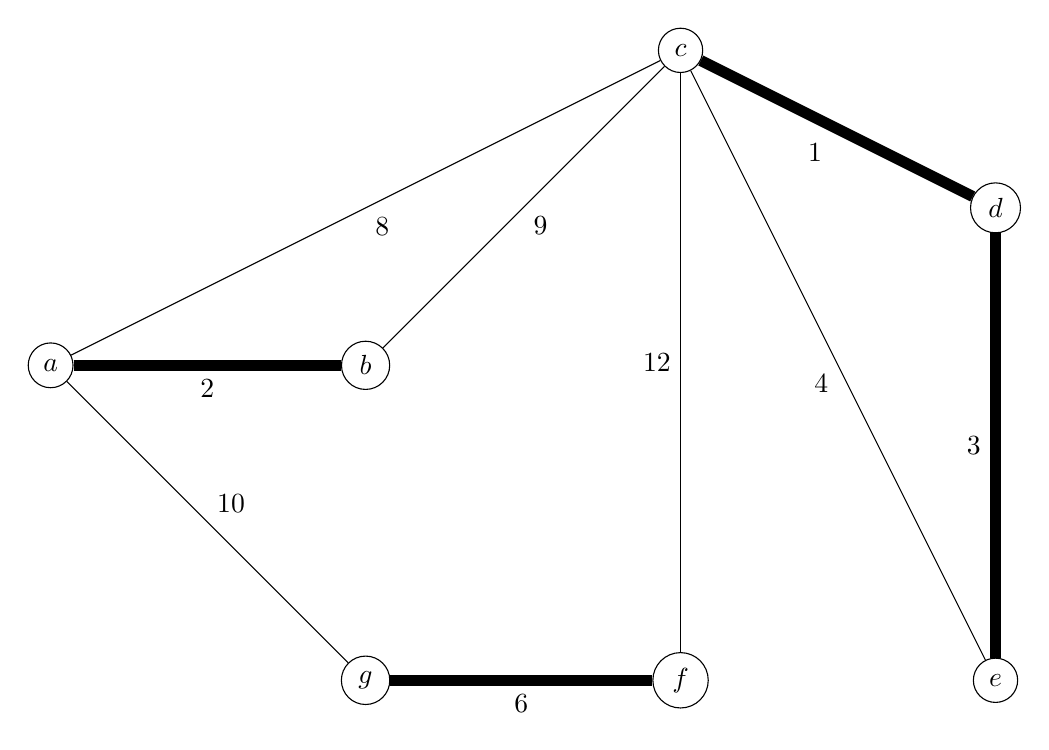
\begin{tikzpicture}[
		wide/.style={line width=4pt},
		vertex/.style={circle,draw,minimum size=16},
		scale=4]
		\node[vertex] (a) at (0,0) {$a$};
		\node[vertex] (b) at (1,0) {$b$};
		\node[vertex] (c) at (2,1) {$c$};
		\node[vertex] (d) at (3,0.5) {$d$};
		\node[vertex] (g) at (1,-1) {$g$};
		\node[vertex] (f) at (2,-1) {$f$};
		\node[vertex] (e) at (3,-1) {$e$};
		\draw[wide] (a) to [edge label'=2] (b); 
		\draw (a) to [edge label'=8] (c); 
		\draw (b) to [edge label'=9] (c); 
		\draw[wide] (c) to [edge label'=1] (d); 
		\draw[wide] (d) to [edge label'=3] (e); 
		\draw (c) to [edge label'=4] (e); 
		\draw (c) to [edge label'=12] (f);
		\draw[wide] (g) to [edge label'=6] (f);
		\draw (g) to [edge label'=10] (a);   
\end{tikzpicture}
\end{center}
\problemend{}
%%%%%%%%%%%%%%%%%%%%%%%%%%%%%%%%%%%%%%%%%%%%%%%%%%%%%%%%%%%%%%%%%%%%%%%%%%%%%%%
% YOUR ANSWER GOES HERE: type yor answer in below                             %
%%%%%%%%%%%%%%%%%%%%%%%%%%%%%%%%%%%%%%%%%%%%%%%%%%%%%%%%%%%%%%%%%%%%%%%%%%%%%%%


%%%%%%%%%%%%%%%%%%%%%%%%%%%%%%%%%%%%%%%%%%%%%%%%%%%%%%%%%%%%%%%%%%%%%%%%%%%%%%%
% A PROBLEM BEGINS HERE                                                       %
%%%%%%%%%%%%%%%%%%%%%%%%%%%%%%%%%%%%%%%%%%%%%%%%%%%%%%%%%%%%%%%%%%%%%%%%%%%%%%%
\skippagesuntil{4}
\problem{}\label{2}
\textbf{Your work for Problem 2 will be divided up into parts (a) and (b) on the following pages. On this page we offer some useful insight and context.} The goal of this problem is to construct an example of a weighted graph $G=(V, E, w)$ where there exists a source vertex $s$ such that Prim's algorithm (starting at $s$) adds the edges of the MST in a different order than Kruskal's algorithm. 

To complete the first part of this problem, we must identify how each algorithm adds edges to the intermediate spanning forest during execution.
That is, we must identify how the edges of the intermediate spanning forests are stored.

Recall that both Prim's and Kruskal's algorithms build an intermediate spanning forest edge-by-edge until it is connected.
The initial intermediate spanning forest in both algorithms is a collection of isolated vertices.
The the two algorithms differ from each other in deciding which edge to add at each step.
Prim's algorithm starts with a source vertex $s$ and always adds a safe edge leaving the component of the current intermediate spanning forest that contains $s$.
Kruskal's algorithm always adds the minimum weight safe edge in the current intermediate spanning forest.
We often say that an edge is ``added to the MST'' when it is added to the intermediate spanning forest because the intermediate spanning forest is a subgraph of the MST. 

In Kruskal's algorithm it is pretty clear when an edge is added to the intermediate spanning forests. 
Observe that we actually add edges to a variable $F$ which stores the edges of the intermediate spanning forest as it grows.

In Prim's algorithm, the story isn't as simple.
Observe that a vertex $x \in V$ is added to the connected component which contains the source vertex $s$ when it is removed from the queue $Q$.
The only exception is the source vertex itself which is already in the appropriate component to begin with. 
Recall that in class and the notes, we argued that each vertex is removed from the queue at most once.
To add a vertex $x$ to the component in the current intermediate spanning forest, we must add an appropriate safe edge to the intermediate spanning forest.
The way we keep track of the edge added is by storing it in $P[x]$. 
More specifically, we assume that once a vertex is added to the component containing $s$ (i.e.\ removed from the queue) then $(P[x], x)$ is added to our intermediate spanning forest.
Observe that we will never update $P[x]$ after vertex $x$ is removed from the queue. 
At any step of the algorithm, we can retrieve the edges in our current intermediate spanning forest by looking at all entries of $P$ that correspond to vertices already removed from the queue.
Note, the source vertex started in the correct connected to begin and so we don't need an edge to add it at any step.
However, one can observe that $P[s] = NULL$ throughout the algorithm. 
This makes sense considering an MST has exactly $|V|-1$ edges. 

In parts (2a) and (2b), using the graph pictured below, assign the weights 1, 2, 3, 4, 5, 6, 7, 8 to the edges of the graph such that every edge gets a different weight. You will need to copy this diagram for both parts (2a) and (2b). \textbf{Note:} Since the edge weights are all distinct, there is only one minimum spanning tree for the graph. So you should get the same minimum spanning tree in both (2a) and (2b). The only difference is that the edges should be added in different orders.
\problemend{}


\begin{center}
	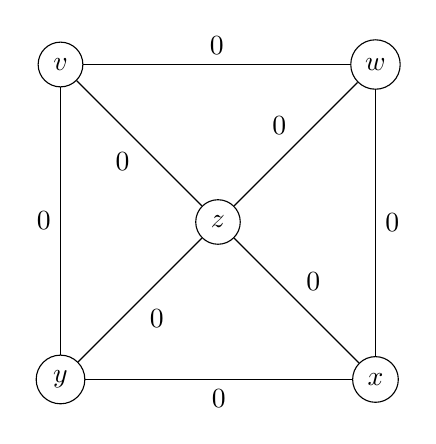
\begin{tikzpicture}[
		wide/.style={line width=4pt},
		vertex/.style={circle,draw,minimum size=16},
		scale=4]
		\node[vertex] (v) at (0,0) {$v$};
		\node[vertex] (w) at (1,0) {$w$};
		\node[vertex] (x) at (1,-1) {$x$};
		\node[vertex] (y) at (0,-1) {$y$};
		\node[vertex] (z) at ($ (v)!0.5!(x) $) {$z$};

		\draw (v) to [edge label'=0] (y); % replace the "0" with a different digit
		\draw (v) to [edge label =0] (w); % replace the "0" with a different digit
		\draw (v) to [edge label'=0] (z); % replace the "0" with a different digit
		\draw (w) to [edge label =0] (x); % replace the "0" with a different digit
		\draw (w) to [edge label'=0] (z); % replace the "0" with a different digit
		\draw (x) to [edge label'=0] (z); % replace the "0" with a different digit
		\draw (x) to [edge label =0] (y); % replace the "0" with a different digit
		\draw (y) to [edge label'=0] (z); % replace the "0" with a different digit
\end{tikzpicture}
\end{center}


\clearpage
\begin{enumerate}
	\myitem[(2a)]\label{2a} 
	Adjust the figure below to display your edge weights, replacing 0 with digits of your choice. Then use Prim's algorithm \emph{as defined in Week7.pdf} to compute the MST\@. For your answer you must give a starting vertex and the order in which Prim's algorithm adds the edges to the MST (that is, adds an edge to the current intermediate spanning forest that will eventually be contained in the MST)\@. \textbf{For each edge added to the MST, clearly indicate both the edge and its weight.}
\end{enumerate}

\problemend{}
%%%%%%%%%%%%%%%%%%%%%%%%%%%%%%%%%%%%%%%%%%%%%%%%%%%%%%%%%%%%%%%%%%%%%%%%%%%%%%%
% YOUR ANSWER GOES HERE: edit the figure and type yor answer below            %
%%%%%%%%%%%%%%%%%%%%%%%%%%%%%%%%%%%%%%%%%%%%%%%%%%%%%%%%%%%%%%%%%%%%%%%%%%%%%%%
\begin{center}
	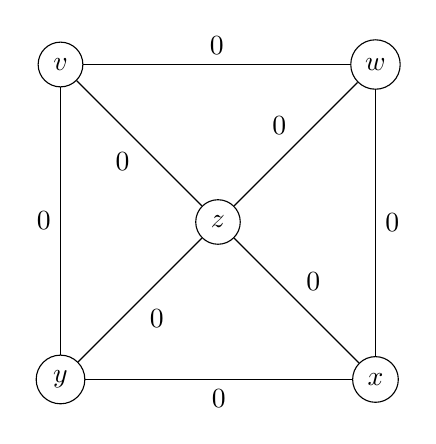
\begin{tikzpicture}[
		wide/.style={line width=4pt},
		vertex/.style={circle,draw,minimum size=16},
		scale=4]
		\node[vertex] (v) at (0,0) {$v$};
		\node[vertex] (w) at (1,0) {$w$};
		\node[vertex] (x) at (1,-1) {$x$};
		\node[vertex] (y) at (0,-1) {$y$};
		\node[vertex] (z) at ($ (v)!0.5!(x) $) {$z$};

		\draw (v) to [edge label'=0] (y); % replace the "0" with a different digit
		\draw (v) to [edge label =0] (w); % replace the "0" with a different digit
		\draw (v) to [edge label'=0] (z); % replace the "0" with a different digit
		\draw (w) to [edge label =0] (x); % replace the "0" with a different digit
		\draw (w) to [edge label'=0] (z); % replace the "0" with a different digit
		\draw (x) to [edge label'=0] (z); % replace the "0" with a different digit
		\draw (x) to [edge label =0] (y); % replace the "0" with a different digit
		\draw (y) to [edge label'=0] (z); % replace the "0" with a different digit
\end{tikzpicture}
\end{center}



\clearpage\skippagesuntil{8}
\begin{enumerate}
	\myitem[(2b)]\label{2b} Adjust the figure below to display your edge weights \emph{which must be the same as for \ref{2a}}, replacing 0 with digits of your choice. Then use Kruskal's algorithm \emph{as defined in Week7.pdf} to compute the MST\@. For your answer you must give the order in which Kruskal's algorithm adds the edges to the MST\@.  \textbf{For each edge added to the MST, clearly indicate both the edge and its weight.} You do not need to specify the state of the algorithm during its execution (i.e.\ we do not need to see the state of the disjoint sets data structure in your answer).
\end{enumerate}
\problemend{}
%%%%%%%%%%%%%%%%%%%%%%%%%%%%%%%%%%%%%%%%%%%%%%%%%%%%%%%%%%%%%%%%%%%%%%%%%%%%%%%
% YOUR ANSWER GOES HERE: edit the figure and type yor answer below            %
%%%%%%%%%%%%%%%%%%%%%%%%%%%%%%%%%%%%%%%%%%%%%%%%%%%%%%%%%%%%%%%%%%%%%%%%%%%%%%%
\begin{center}
	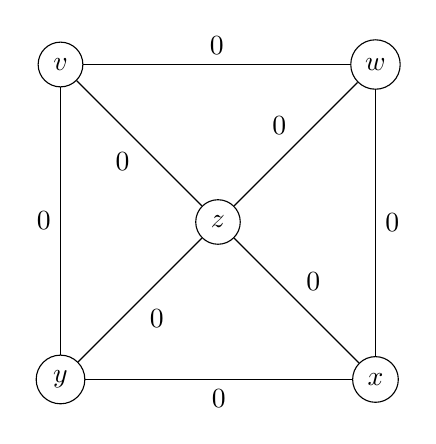
\begin{tikzpicture}[
		wide/.style={line width=4pt},
		vertex/.style={circle,draw,minimum size=16},
		scale=4]
		\node[vertex] (v) at (0,0) {$v$};
		\node[vertex] (w) at (1,0) {$w$};
		\node[vertex] (x) at (1,-1) {$x$};
		\node[vertex] (y) at (0,-1) {$y$};
		\node[vertex] (z) at ($ (v)!0.5!(x) $) {$z$};

		\draw (v) to [edge label'=0] (y); % replace the "0" with a different digit
		\draw (v) to [edge label =0] (w); % replace the "0" with a different digit
		\draw (v) to [edge label'=0] (z); % replace the "0" with a different digit
		\draw (w) to [edge label =0] (x); % replace the "0" with a different digit
		\draw (w) to [edge label'=0] (z); % replace the "0" with a different digit
		\draw (x) to [edge label'=0] (z); % replace the "0" with a different digit
		\draw (x) to [edge label =0] (y); % replace the "0" with a different digit
		\draw (y) to [edge label'=0] (z); % replace the "0" with a different digit
\end{tikzpicture}
\end{center}



\end{document}

%%%%%%%%%%%%%%%%%%%%%%%%%%%%%%%%%%%%%%%%%%%%%%%%%%%%%%%%%%%%%%%%%%%%%%%%%%%%%%%
% STANDARDS                                                                   %
%%%%%%%%%%%%%%%%%%%%%%%%%%%%%%%%%%%%%%%%%%%%%%%%%%%%%%%%%%%%%%%%%%%%%%%%%%%%%%%

% 1. Loop invariants and proof by induction
% 2. Asymptotic notation
% 3. Asymptotic analysis I: correctly writing down equations for counting operations given pseudocode with simple independent loops
% 4. Asymptotic analysis II: correctly writing down equations for counting operations given pseudocode with nested dependent loops
% 5. Recurrence relations I: write down correct recurrence for a recursive algorithm
% 6. Recurrence relations II: solve by unrolling
% 7. Recurrence relations III: solve by tree method
% 8. Divide and conquer: important principles (when does it apply and when not)
% 9. Average case analysis (of quicksort), compare to worst-case behavior
% 10. Hash tables: collisions, load factor, when to apply vs balanced binary tree
% 11. Greedy algorithms I: exchange argument for correctness (mastery can be demonstrated either using interval scheduling or Huffman coding)
% 12. Greedy algorithms II: examples where greedy algorithms do not work
% 13. Shortest paths I: breadth-first search for unweighted graphs
% 14. Shortest paths II: Dijkstra’s algorithm (or Bellman–Ford which we cover later)
% 15. Minimum spanning trees I: safe and useless edges
% 16. Minimum spanning trees II: the generic algorithm and at least one of Kruskal’s or Prim’s algorithm
% 17. Max flow min cut I: residual graph
% 18. Max flow min cut II: applying max flow (reducing to max flow, e.g. bipartite matching)
% 19. Dynamic programming I: principles (when does it apply and when not)
% 20. Dynamic programming II: rigorous understanding of a simple 1-dimensional example(Fibonacci numbers or rod cutting)
% 21. Dynamic programming III: write down recurrence for computing local solution in a complex example (e.g. edit distance)
% 22. Dynamic Programming IV: order of subproblems and topological sort
% 23. Dynamic Programming V: backtracking (recovering the optimal solution not just its value)
% 24. Complexity theory: basic definitions (P, NP, NP-hard, NP-complete, reduction)